\begin{figure}[H]
    \centering
    \definecolor{polytropered}{RGB}{180,45,55}
    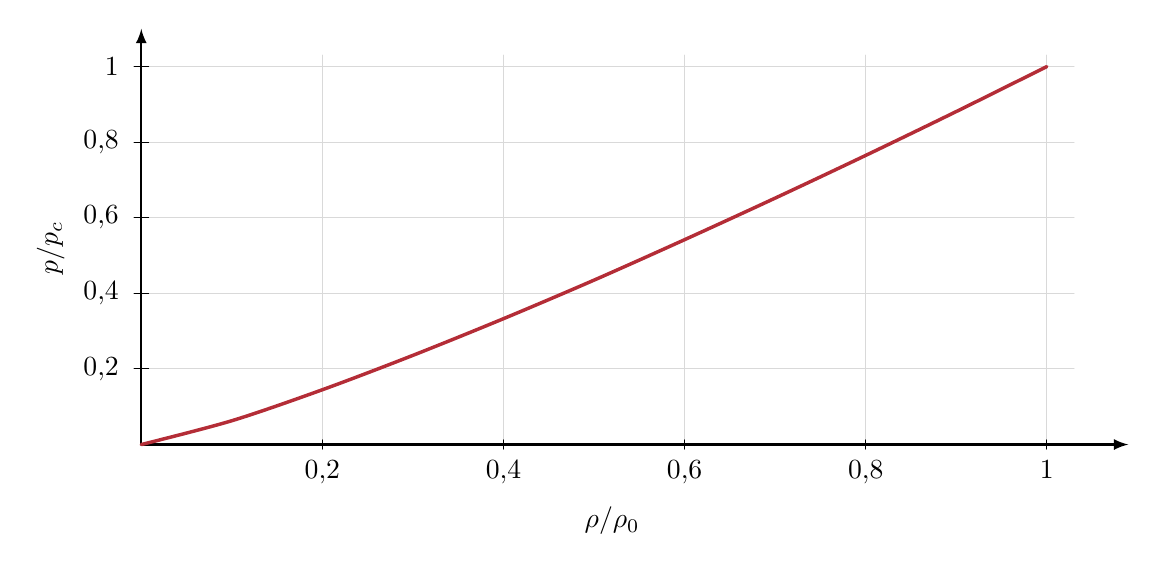
\begin{tikzpicture}[x=11.5cm,y=4.8cm,line cap=round,line join=round]
        \foreach \x in {0.2,0.4,0.6,0.8,1.0} {
            \draw[black!15] (\x,0) -- (\x,1.03);
        }
        \foreach \y in {0.2,0.4,0.6,0.8,1.0} {
            \draw[black!15] (0,\y) -- (1.03,\y);
        }
        \draw[-latex,line width=0.8pt] (0,0) -- (1.09,0);
        \draw[-latex,line width=0.8pt] (0,0) -- (0,1.10);

        \draw[polytropered,line width=1.25pt,smooth]
            plot coordinates {
                (0,0) (0.1,0.063) (0.2,0.145) (0.3,0.236)
                (0.4,0.333) (0.5,0.435) (0.6,0.542)
                (0.7,0.652) (0.8,0.765) (0.9,0.881) (1,1)
            };

        \node[anchor=north] at (0.52,-0.14) {$\rho/\rho_0$};
        \node[rotate=90] at (-0.10,0.52) {$p/p_c$};

        \foreach \x/\lab in {0.2/{0{,}2},0.4/{0{,}4},0.6/{0{,}6},0.8/{0{,}8},1/{1}} {
            \draw (\x,0.012) -- (\x,-0.012);
            \node[anchor=north] at (\x,-0.018) {$\lab$};
        }
        \foreach \y/\lab in {0.2/{0{,}2},0.4/{0{,}4},0.6/{0{,}6},0.8/{0{,}8},1/{1}} {
            \draw (0.008,\y) -- (-0.008,\y);
            \node[anchor=east] at (-0.014,\y) {$\lab$};
        }
    \end{tikzpicture}
    \caption{Relación barotrópica entre presión y densidad para la politropa de índice $n=5$.}
\end{figure}
